\section{Problema a resolver}

En este trabajo se intentará resolver el problema de clasificación del conjunto de datos South German Credit. Este conjunto de datos cuenta con 21 variables, siendo la última de estas la variable a predecir. La variable a predecir se trata de una variable lógica, sobre si se ha cumplido o no los pagos del crédito concedido.

Este conjunto de datos cuenta con información sobre la persona que solicita el crédito, por ejemplo el estado de la cuenta bancaria, si ha cumplido o no con los pagos de otros créditos con anterioridad, el trabajo, la edad, entre otras variables, y debido a la gran cantidad de estas, se aplicará un análisis de componentes principales (PCA) de cara a reducir la dimensionalidad del problema.

Para entender de una mejor forma el conjunto de datos, se han realizado distintas gráficas para mostrar el comportamiento de cada predictor.

Lo primero que tenemos que tener en cuenta para un problema de clasificación es si el problema está balanceado, es decir, contamos con un número similar de observaciones de cada clase:

\begin{figure}[H]
	\centering
	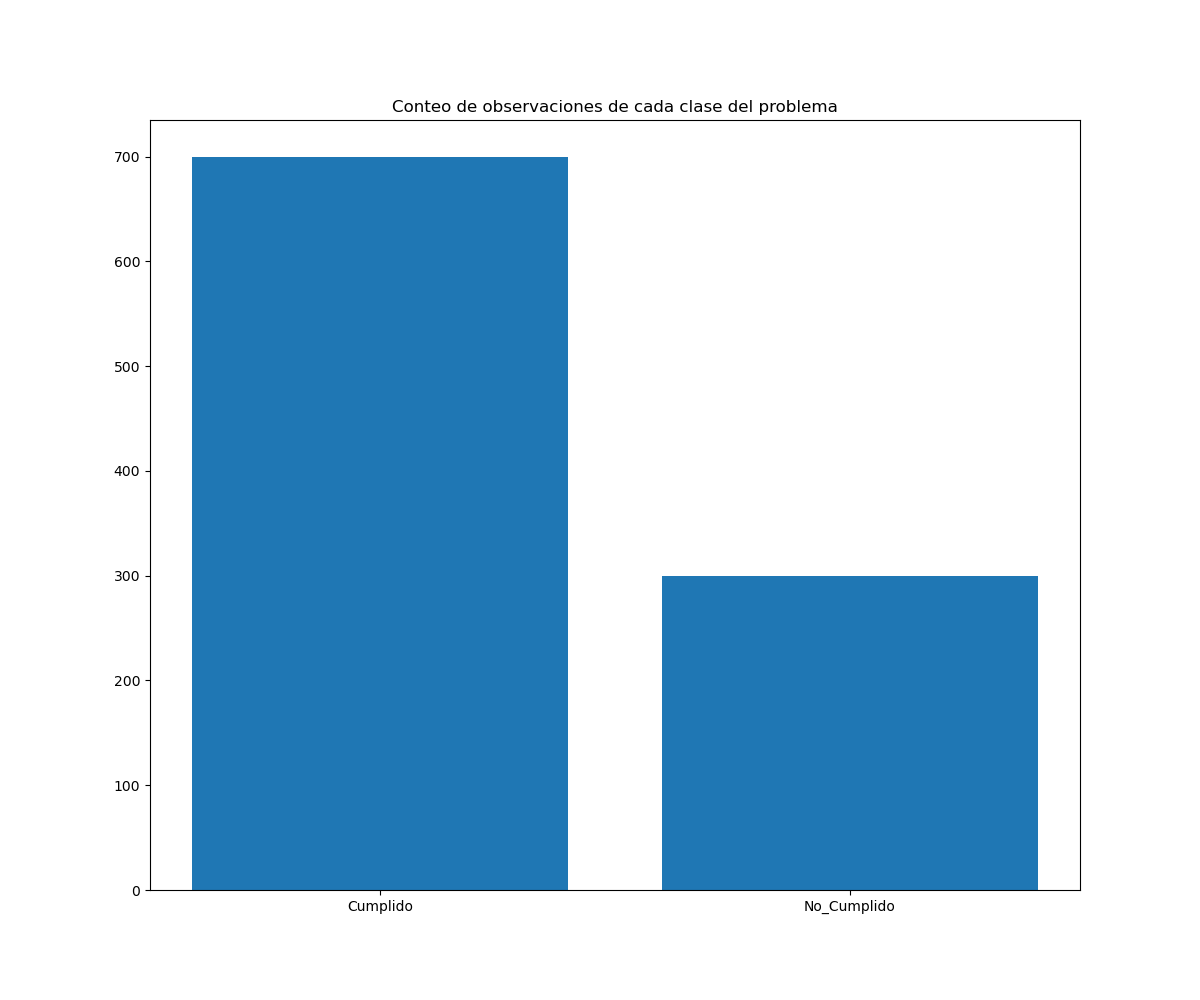
\includegraphics[scale = 0.6]{conteo_clases.png}
	\caption{Conteo de observaciones para cada clase del problema.}
	\label{fig:conteo_clases}
\end{figure}

Como podemos ver, en este caso no contamos con un número similar de observaciones en cada clase, teniendo en la clase donde no se han cumplido los pagos menos de la mitad de observaciones que en la clase donde si. Este problema lo podríamos solucionar intentando obtener más muestras o aplicando un sobremuestreo con técnicas como SMOTE o ADASYN, sin embargo no es el objetivo de la asignatura y por lo tanto se ha trabajado con el conjunto dado.

También se ha obtenido la matriz de correlaciones entre predictores, ya que es interesante saber si dos predictores están muy correlados de cara a saber si aportan la misma información y por lo tanto podríamos eliminar uno de ellos:

\begin{figure}[H]
	\centering
	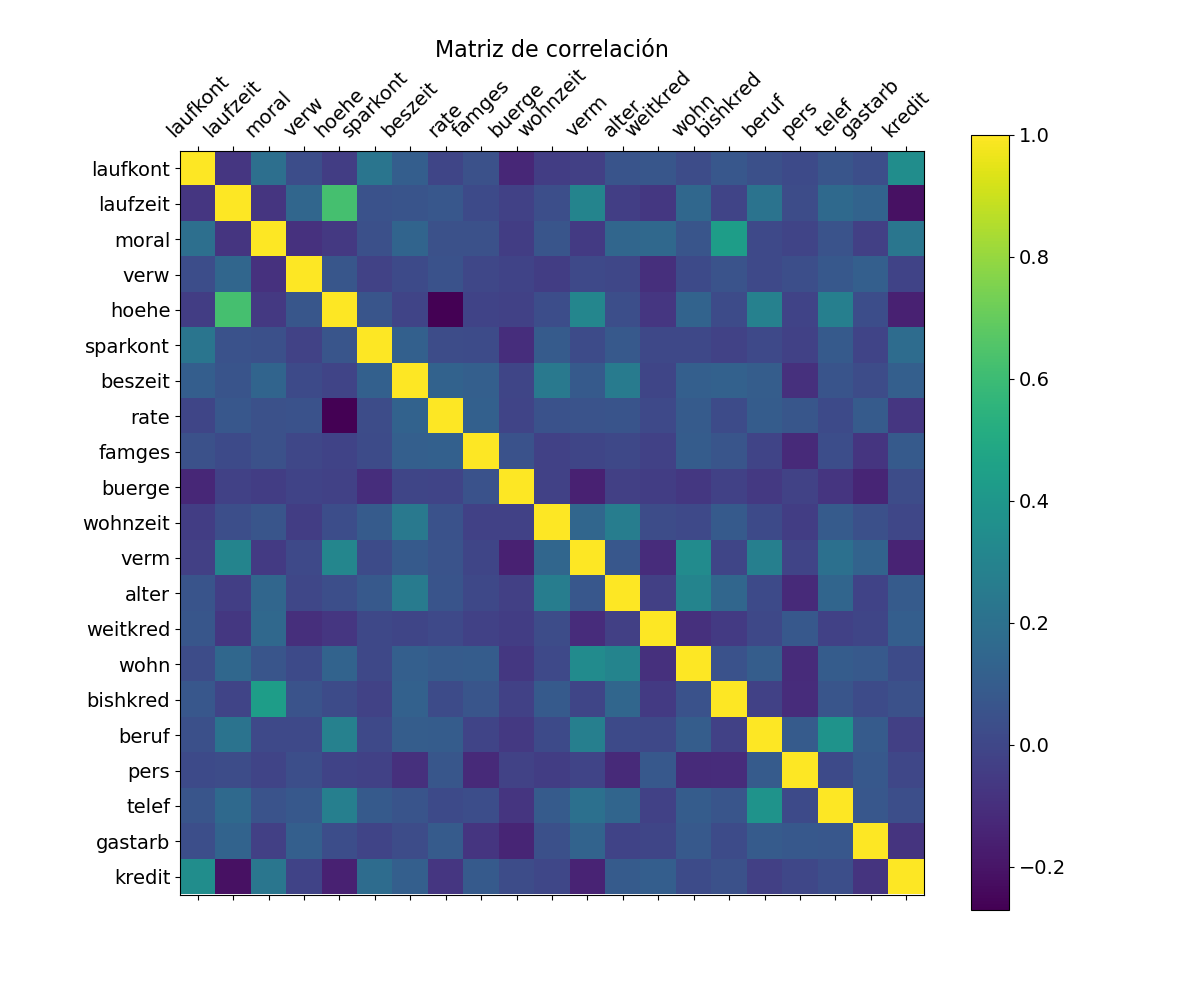
\includegraphics[scale = 0.6]{matriz_correlacion.png}
	\caption{Matriz de correlación entre las variables del problema.}
	\label{fig:matriz_correlacion}
\end{figure}

En este caso no existe una correlación muy alta entre ninguno de los predictores.

Otra de las gráficas de interés obtenidas es una gráfica con la distribución de cada predictor, ya que en este caso vamos a aplicar PCA, técnica que asume que las variables siguen una distribución normal y, aunque podemos aplicar esta técnica sin que esto se cumpla, obtendremos mejores resultados si esto es cierto:

\begin{figure}[H]
	\centering
	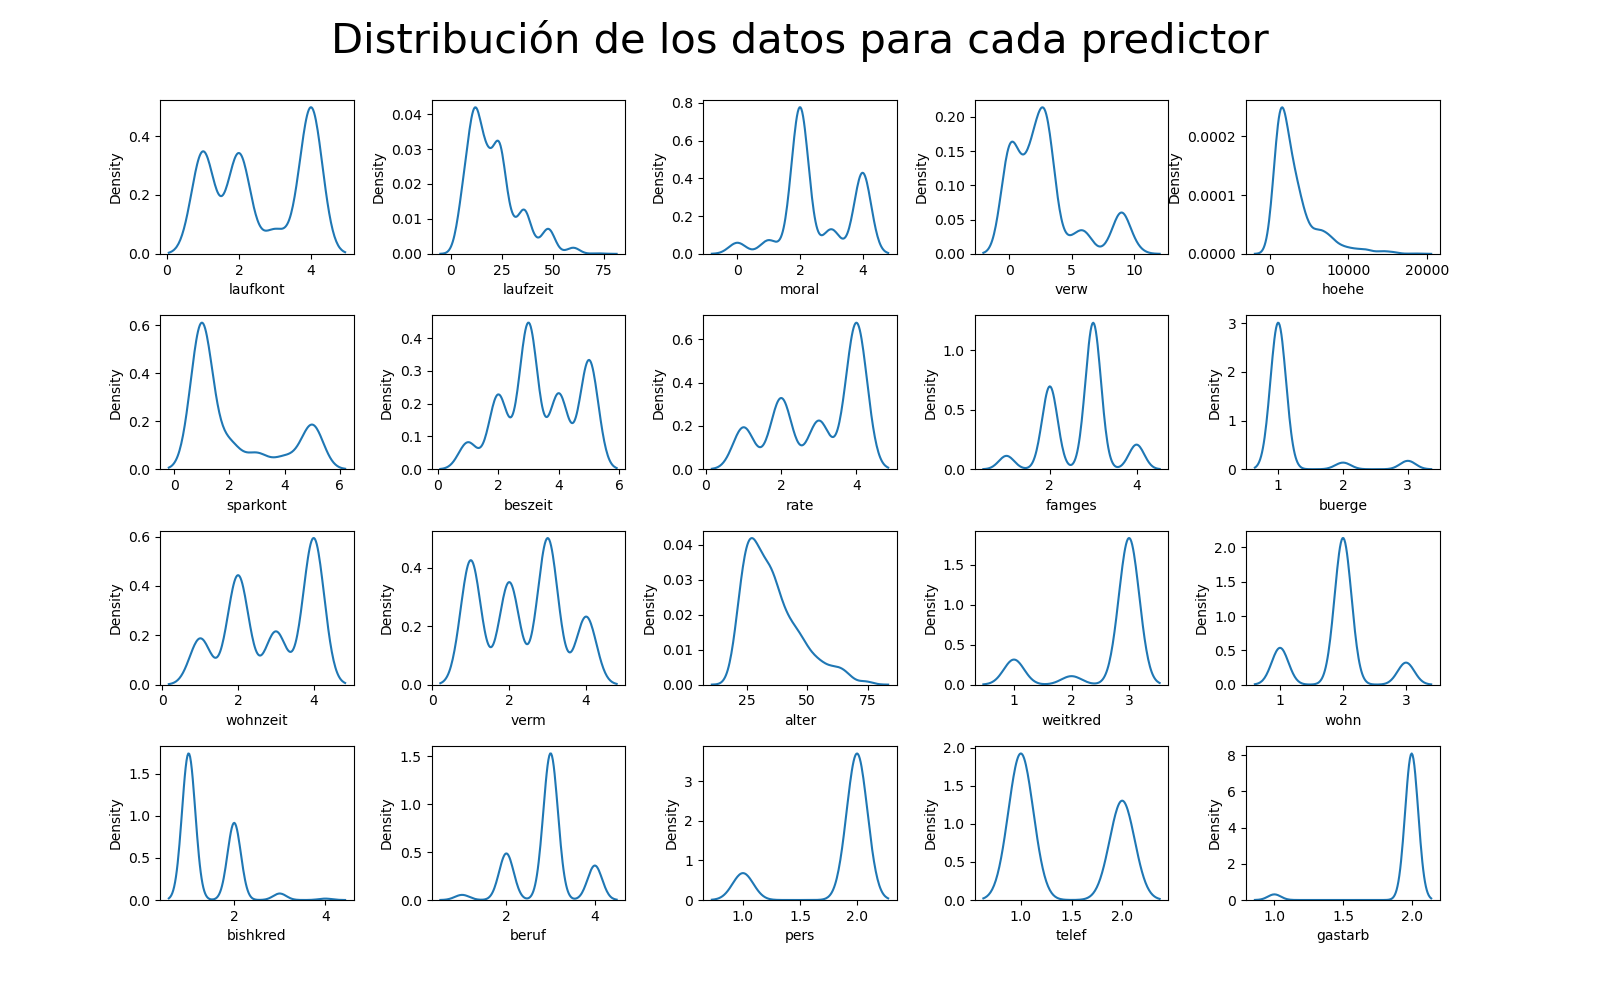
\includegraphics[scale = 0.4]{distribucion_variables.png}
	\caption{Distribución de las variables del problema.}
	\label{fig:distribucion_variables}
\end{figure}

Para nuestro problema vemos que ninguno de nuestros predictores sigue una distribución normal, aunque aun así vamos a intentar aplicar la reducción de dimensionalidad con PCA.



\newpage
